
\begin{figure}[t]%h!
    \centering
    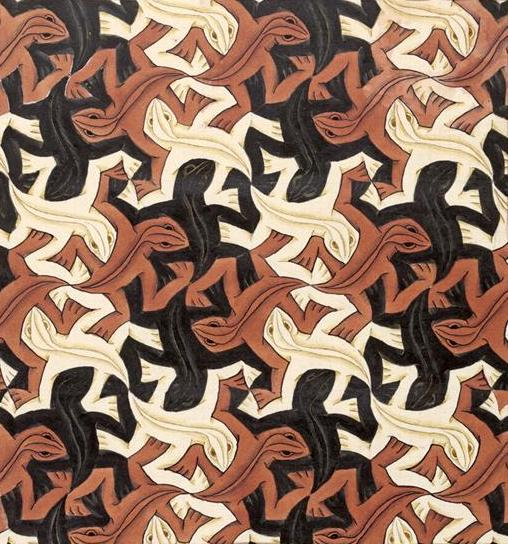
\includegraphics[width=0.4\linewidth]{lizard-1.jpg}
    \caption{A monohedral tiling of the plane using a Lizard-shaped tile by artist M.C Escher \cite{m.c.escherLizard1942}. Although the lizards are colored differently, they are, in fact, the same tile. Although the coloring of the lizards is different, they are all the same tile.}
    \label{fig:tiling_three}
\end{figure}


\mycomment{  %! Block comment
\begin{figure}[t]%h!
    \centering
    \begin{subfigure}{.47\textwidth}
        \centering
        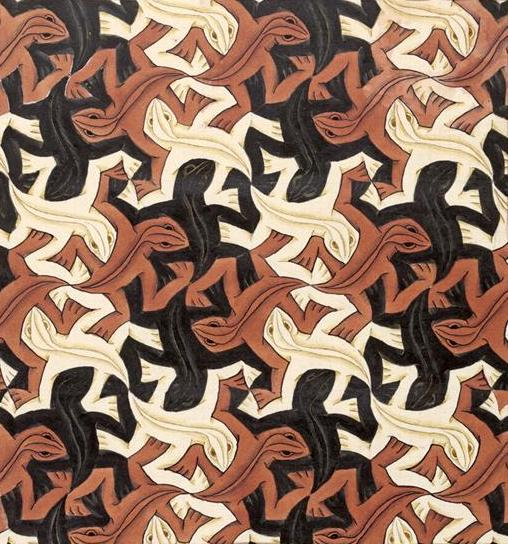
\includegraphics[width=0.9\linewidth]{lizard-1.jpg}
        \caption{Lizard}
        %\label{fig:tiling_three}
    \end{subfigure}\quad
    \begin{subfigure}{.47\textwidth}
        \centering
        
\includegraphics[width=0.9\linewidth]{flying-fish.jpg}
        \caption{Flying fish}
        \label{fig:tiling_four}
    \end{subfigure}
    \caption{from \cite{m.c.escherLizard1942}}
    \label{fig:tilingsss_two}
\end{figure}
}